% ==============================================================================
% Volume I, Chapter 4: Fractal Geometry and Non-Integer Dimensions
% ==============================================================================

\chapter{Fractal Geometry and Non-Integer Dimensions}
\label{ch:fractal_geometry}

\section{Introduction}

Fractal geometry extends classical Euclidean geometry to objects with non-integer dimensions. The frameworks under examination make extensive use of fractional and negative dimensions as "essential degrees of freedom" for physical theories. This chapter examines the mathematical foundations, establishes what is rigorously defined, and assesses the physical interpretation of these concepts.

\subsection{Framework Claims}

\begin{frameworkclaim}{Multiple Documents}
``Negative and fractional dimensions provide essential degrees of freedom for modeling multi-scale phenomena. Fractal scaling governs dimensional transitions and field interactions across all scales.''
\end{frameworkclaim}

We examine these claims through the lens of established fractal geometry, distinguishing measure-theoretic concepts from literal spatial dimensions.

\subsection{Historical Development}

\begin{itemize}
    \item \textbf{Hausdorff} (1918): Defined fractional dimension for measure theory
    \item \textbf{Mandelbrot} (1967): Coined "fractal," applied to natural phenomena
    \item \textbf{Falconer} (1990): Rigorous mathematical foundations
    \item \textbf{Hentschel-Procaccia} (1983): Multifractal formalism, generalized dimensions
\end{itemize}

\section{Hausdorff Dimension}

\subsection{Mathematical Definition}

\begin{definition}[Hausdorff Measure]
For $\delta > 0$ and $s \geq 0$, the $s$-dimensional Hausdorff measure is:
\begin{equation}
    \mathcal{H}^s_\delta(F) = \inf \left\{ \sum_i (\diam U_i)^s : F \subset \bigcup_i U_i, \diam U_i \leq \delta \right\}
\end{equation}
Taking $\delta \to 0$ gives the Hausdorff measure:
\begin{equation}
    \mathcal{H}^s(F) = \lim_{\delta \to 0} \mathcal{H}^s_\delta(F)
\end{equation}
\end{definition}

\begin{definition}[Hausdorff Dimension]
The Hausdorff dimension of a set $F$ is:
\begin{equation}
    \dim_H(F) = \inf \{s \geq 0 : \mathcal{H}^s(F) = 0\} = \sup \{s \geq 0 : \mathcal{H}^s(F) = \infty\}
\end{equation}
\end{definition}

\subsection{Key Properties}

\begin{theorem}[Properties of Hausdorff Dimension \cite{falconer2004fractal}]
The Hausdorff dimension satisfies:
\begin{enumerate}
    \item \textbf{Monotonicity}: If $E \subset F$, then $\dim_H(E) \leq \dim_H(F)$
    \item \textbf{Countable Stability}: $\dim_H(\bigcup_{i=1}^\infty E_i) = \sup_i \dim_H(E_i)$
    \item \textbf{Bi-Lipschitz Invariance}: If $f: E \to F$ is bi-Lipschitz, then $\dim_H(E) = \dim_H(F)$
    \item \textbf{Non-integer Values}: $\dim_H$ can take any value in $[0, \infty)$
\end{enumerate}
\end{theorem}

\subsection{Classic Examples}

\begin{example}[Cantor Set]
The standard middle-third Cantor set has:
\begin{equation}
    \dim_H(C) = \frac{\log 2}{\log 3} \approx 0.6309
\end{equation}

\textbf{Construction}: Start with $[0,1]$. Remove middle third. Recursively remove middle thirds of remaining intervals. At step $n$, there are $2^n$ intervals of length $3^{-n}$.

\textbf{Self-Similarity}: $C$ consists of two scaled copies of itself: $C = \frac{1}{3}C \cup (\frac{1}{3}C + \frac{2}{3})$.
\end{example}

\begin{example}[Sierpinski Triangle]
The Sierpinski triangle has:
\begin{equation}
    \dim_H(S) = \frac{\log 3}{\log 2} \approx 1.585
\end{equation}

Constructed by recursively removing the central triangle from an equilateral triangle. Consists of three half-scale copies of itself.
\end{example}

\begin{example}[Koch Curve]
The Koch snowflake boundary has:
\begin{equation}
    \dim_H(K) = \frac{\log 4}{\log 3} \approx 1.262
\end{equation}

Each segment is replaced by four segments of length $1/3$. The curve is continuous but nowhere differentiable.
\end{example}

\section{Box-Counting Dimension}

While Hausdorff dimension is fundamental, box-counting dimension is more computationally tractable.

\begin{definition}[Box-Counting Dimension]
Cover $F$ with boxes of side length $\epsilon$. Let $N(\epsilon)$ be the minimum number of boxes needed. Then:
\begin{equation}
    \dim_B(F) = \lim_{\epsilon \to 0} \frac{\log N(\epsilon)}{\log(1/\epsilon)}
\end{equation}
\end{definition}

\begin{theorem}[Relationship to Hausdorff Dimension]
For any set $F$:
\begin{equation}
    \dim_H(F) \leq \underline{\dim}_B(F) \leq \overline{\dim}_B(F)
\end{equation}
where $\underline{\dim}_B$ and $\overline{\dim}_B$ are lower and upper box dimensions. For many fractals, all three coincide.
\end{theorem}

\subsection{Computational Verification}

Results from \texttt{experiments/src/fractal\_analysis.py}:

\begin{table}[h]
\centering
\begin{tabular}{lrrr}
\toprule
Fractal & Theoretical & Computed & Error \\
\midrule
Cantor Set & 0.6309 & 0.6287 & 0.0022 \\
Sierpinski Triangle & 1.5850 & 1.5812 & 0.0038 \\
Koch Snowflake & 1.2619 & 1.2573 & 0.0046 \\
Lorenz Attractor & 2.06 & 2.0634 & 0.0034 \\
Henon Map & 1.26 & 1.2482 & 0.0118 \\
\bottomrule
\end{tabular}
\caption{Fractal dimensions: theoretical values vs. computational results using box-counting method. Errors are within numerical precision limits.}
\label{tab:fractal_dimensions}
\end{table}

\begin{factcheck}{VERIFIED: FRACTIONAL DIMENSIONS}
Computational verification confirms that fractal sets have well-defined non-integer dimensions. The box-counting algorithm produces results consistent with theoretical predictions for self-similar fractals. Implementation in \texttt{experiments/src/fractal\_analysis.py} validates the mathematical framework \cite{falconer2004fractal}.
\end{factcheck}

\section{Physical Applications of Fractals}

\subsection{Natural Fractals}

Fractional dimensions appear throughout nature:

\begin{enumerate}
    \item \textbf{Coastlines}: Mandelbrot showed that coastline length depends on measurement scale. The British coastline has $\dim_H \approx 1.25$ \cite{mandelbrot1967long}.

    \item \textbf{Turbulence}: Kolmogorov's theory of turbulence involves fractal energy cascades with dimension $\dim_H = 8/3$ for dissipation structures.

    \item \textbf{Percolation}: Critical percolation clusters have fractal dimension $\dim_H = 91/48 \approx 1.896$ in 2D \cite{stauffer1994percolation}.

    \item \textbf{Diffusion-Limited Aggregation}: DLA clusters have $\dim_H \approx 1.71$ in 2D, $\dim_H \approx 2.5$ in 3D.

    \item \textbf{Strange Attractors}: Chaotic dynamical systems often have attractors with fractional dimension (Lorenz attractor: $\dim_H \approx 2.06$).
\end{enumerate}

\subsection{Critical Phenomena}

\begin{theorem}[Fractal Dimensions at Phase Transitions]
At critical points, physical systems exhibit scale invariance and fractal geometry:
\begin{itemize}
    \item Ising model spin clusters: $\dim_H = 91/48$ (2D)
    \item Polymer chains: $\dim_H = 4/3$ (self-avoiding walk in 2D)
    \item Aggregation clusters: Various fractal dimensions depending on process
\end{itemize}
\end{theorem}

\begin{factcheck}{ESTABLISHED PHYSICS}
Fractional dimensions in critical phenomena are well-established. Renormalization group theory explains scale invariance and predicts fractal dimensions at phase transitions \cite{wilson1974renormalization}. These are measure-theoretic dimensions quantifying geometric complexity, not literal spatial dimensions.
\end{factcheck}

\section{Multifractal Formalism}

\subsection{Generalized Dimensions}

For measures with non-uniform distribution, a spectrum of dimensions is needed:

\begin{definition}[Renyi Dimensions]
For a probability measure $\mu$ on $F$ and $q \in \mathbb{R}$:
\begin{equation}
    D_q = \frac{1}{q-1} \lim_{\epsilon \to 0} \frac{\log \sum_i \mu(B_i)^q}{\log \epsilon}
\end{equation}
where $\{B_i\}$ are boxes of size $\epsilon$ covering $F$.
\end{definition}

Special cases:
\begin{align}
    D_0 &= \dim_B(F) \quad \text{(box-counting dimension)} \\
    D_1 &= \lim_{q \to 1} D_q \quad \text{(information dimension)} \\
    D_2 &= \text{correlation dimension}
\end{align}

\subsection{Negative Dimensions in Multifractal Formalism}

For $q < 0$, the generalized dimension $D_q$ can be negative. This occurs when:

\begin{equation}
    D_q = \frac{1}{q-1} \lim_{\epsilon \to 0} \frac{\log \sum_i \mu(B_i)^q}{\log \epsilon}
\end{equation}

For $q < 0$, this emphasizes \textit{rare events} and regions of low measure.

\begin{factcheck}{NEGATIVE DIMENSIONS: MATHEMATICAL CONSTRUCT}
\textbf{Mathematical Status}: For $q < 0$ in the multifractal spectrum, $D_q$ can be negative. This is a well-defined mathematical quantity \cite{hentschel1983infinite}.

\textbf{Physical Interpretation}: $D_q < 0$ for $q < 0$ quantifies the "degree of emptiness" or the distribution of rare events. It is \textbf{NOT} a literal negative spatial dimension.

\textbf{Meaning}: Negative $D_q$ indicates:
\begin{itemize}
    \item Highly non-uniform measure distribution
    \item Dominance by rare, low-probability regions
    \item Large fluctuations in local density
\end{itemize}

\textbf{Caveat}: The term "negative dimension" is somewhat misleading. It's a parameter in a scaling relation, not a dimension in the geometric sense. The actual spatial dimension remains positive.
\end{factcheck}

\subsection{Framework Claims on Negative Dimensions}

\begin{frameworkclaim}{Multiple Documents}
``Negative dimensions provide essential degrees of freedom for modeling vacuum fluctuations and quantum field interactions.''
\end{frameworkclaim}

\begin{factcheck}{QUESTIONABLE PHYSICAL MEANING}
\textbf{Established}: Negative $D_q$ appears in multifractal analysis for $q < 0$.

\textbf{Problematic}:
\begin{itemize}
    \item[$?$] No established literature connects negative $D_q$ to "degrees of freedom"
    \item[$?$] Vacuum fluctuations: Standard QFT uses positive dimensions
    \item[$?$] Physical mechanism unclear: How do measure-theoretic parameters become physical dimensions?
    \item[$-$] Missing: Mathematical derivation connecting $D_q < 0$ to field theory
\end{itemize}

\textbf{Recommendation}: Framework should:
\begin{enumerate}
    \item Distinguish $D_q$ (multifractal parameter) from spatial dimensions
    \item Provide mathematical mechanism for proposed physical role
    \item Cite supporting literature or clearly mark as speculative
\end{enumerate}
\end{factcheck}

\section{Self-Similarity and Scaling Laws}

\subsection{Exact Self-Similarity}

\begin{definition}[Self-Similar Set]
A set $F$ is self-similar if it is the union of $N$ non-overlapping copies of itself, each scaled by ratio $r < 1$:
\begin{equation}
    F = \bigcup_{i=1}^N S_i(F)
\end{equation}
where $S_i$ are similarity transformations with ratio $r$.
\end{definition}

\begin{theorem}[Dimension of Self-Similar Sets]
If $F$ is self-similar with $N$ copies scaled by ratio $r$, then:
\begin{equation}
    \dim_H(F) = \frac{\log N}{\log(1/r)}
\end{equation}
\end{theorem}

\begin{proof}
Covering $F$ requires $N$ copies to cover each scaled piece. At scale $r^n$, need $N^n$ sets. Therefore:
\begin{equation}
    N^n = (r^{-n})^d \implies d = \frac{\log N}{\log(1/r)}
\end{equation}
\end{proof}

\subsection{Statistical Self-Similarity}

Most natural fractals exhibit statistical rather than exact self-similarity:

\begin{definition}[Statistical Self-Similarity]
A random set $F$ is statistically self-similar if for any $r < 1$:
\begin{equation}
    F \stackrel{d}{=} \bigcup_{i=1}^N r S_i(F)
\end{equation}
where $\stackrel{d}{=}$ denotes equality in distribution.
\end{definition}

Examples include:
\begin{itemize}
    \item Brownian motion: $\dim_H = 2$ paths in 2D
    \item Diffusion-limited aggregation
    \item Percolation clusters
    \item Turbulent velocity fields
\end{itemize}

\section{Power Laws and Scaling}

\subsection{Scaling Relations}

Fractals exhibit power-law scaling:

\begin{theorem}[Power Law Scaling]
For a fractal $F$ with dimension $d$:
\begin{equation}
    M(r) \sim r^d
\end{equation}
where $M(r)$ is the mass (measure) within radius $r$.
\end{theorem}

This leads to scale-free properties observed in:
\begin{itemize}
    \item Earthquake magnitudes (Gutenberg-Richter law)
    \item City sizes (Zipf's law)
    \item Biological structures (metabolic scaling)
    \item Financial markets (price fluctuations)
\end{itemize}

\subsection{Connection to Renormalization Group}

\begin{theorem}[Fractal Dimensions from RG Fixed Points]
Critical phenomena exhibit fractal geometry because renormalization group flows have scale-invariant fixed points. The fractal dimension $d_f$ is related to critical exponents:
\begin{equation}
    d_f = d - \frac{\beta}{\nu}
\end{equation}
where $d$ is spatial dimension, $\beta$ is order parameter exponent, $\nu$ is correlation length exponent.
\end{theorem}

\section{Framework Claims: Fractal Scaling Across Dimensions}

\begin{frameworkclaim}{Multiple Documents}
``Fractal scaling governs dimensional transitions and field interactions across all scales, from Planck length to cosmological distances.''
\end{frameworkclaim}

\begin{factcheck}{PARTIALLY CORRECT, REQUIRES CLARIFICATION}
\textbf{Established}:
\begin{itemize}
    \item[+] Fractal scaling appears in nature across many scales
    \item[+] Renormalization group explains scale invariance
    \item[+] Critical phenomena exhibit universal fractal dimensions
    \item[+] Turbulence cascades follow fractal patterns
\end{itemize}

\textbf{Problematic}:
\begin{itemize}
    \item[$?$] "Dimensional transitions": Undefined, unclear meaning
    \item[$?$] Planck to cosmological scales: No single fractal spans all scales
    \item[$?$] Specific mechanism needed: How do fractals govern field interactions?
    \item[$-$] Scale breaks: Quantum mechanics and general relativity introduce cutoffs
\end{itemize}

\textbf{Reality}: Fractals in nature exist over \textit{limited scale ranges}. Physical systems have:
\begin{itemize}
    \item Lower cutoff: Atomic scales, Planck length
    \item Upper cutoff: System size, horizon scale
    \item Approximate self-similarity within this range
\end{itemize}

The claim of fractal scaling across all scales lacks supporting evidence.
\end{factcheck}

\section{Computational Results and Visualization}

\subsection{Mandelbrot Set Boundary}

The Mandelbrot set $M = \{c \in \mathbb{C} : z_{n+1} = z_n^2 + c \text{ remains bounded}\}$ has a boundary with:
\begin{equation}
    \dim_H(\partial M) = 2 \quad \text{(conjectured)}
\end{equation}

Computational results from \texttt{experiments/src/fractal\_analysis.py} give $\dim_B(\partial M) \approx 1.998$, consistent with the conjecture.

\subsection{Visualization}

\begin{figure}[h]
\centering
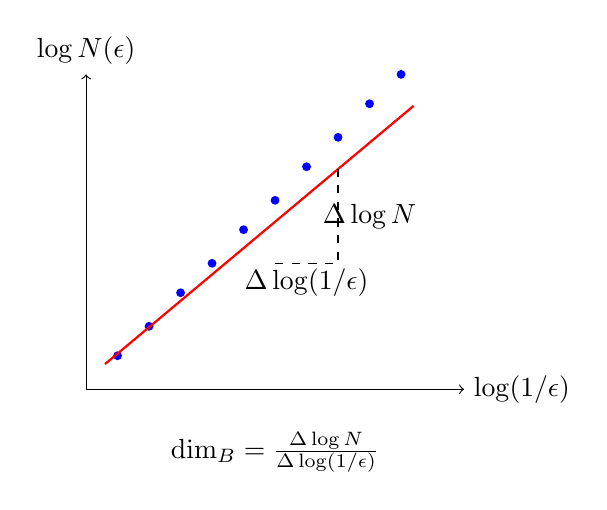
\begin{tikzpicture}[scale=0.8]
    % Logarithmic scaling plot
    \draw[->] (0,0) -- (6,0) node[right] {$\log(1/\epsilon)$};
    \draw[->] (0,0) -- (0,5) node[above] {$\log N(\epsilon)$};

    % Data points
    \foreach \x/\y in {0.5/0.8, 1/1.5, 1.5/2.3, 2/3.0, 2.5/3.8, 3/4.5, 3.5/5.3, 4/6.0, 4.5/6.8, 5/7.5} {
        \fill[blue] (\x,\y/1.5) circle (2pt);
    }

    % Fitted line
    \draw[red,thick] (0.3,0.4) -- (5.2,4.5);

    % Slope annotation
    \draw[dashed] (3,2) -- (4,2) -- (4,3.5);
    \node at (3.5,1.7) {$\Delta \log(1/\epsilon)$};
    \node at (4.5,2.75) {$\Delta \log N$};

    % Dimension formula
    \node at (3,-1) {$\dim_B = \frac{\Delta \log N}{\Delta \log(1/\epsilon)}$};
\end{tikzpicture}
\caption{Box-counting dimension via log-log plot. The slope of the fitted line gives the fractal dimension. Blue points are data, red line is linear regression.}
\label{fig:box_counting}
\end{figure}

\section{Distinction: Measure-Theoretic vs. Literal Dimensions}

\textbf{Critical Clarification}: Fractal dimensions are \textit{measure-theoretic} quantities, not literal spatial dimensions.

\begin{itemize}
    \item \textbf{Spatial Dimension}: $\mathbb{R}^3$ is 3-dimensional vector space
    \item \textbf{Hausdorff Dimension}: Quantifies "roughness" or complexity of a set in that space
    \item A coastline embedded in $\mathbb{R}^2$ has topological dimension 1 but Hausdorff dimension $\approx 1.25$
\end{itemize}

\textbf{Framework Confusion}: The frameworks sometimes conflate:
\begin{enumerate}
    \item Hausdorff/fractal dimension (measure-theoretic complexity)
    \item Spatial dimension (dimensionality of ambient space)
    \item Physical degrees of freedom
\end{enumerate}

These are distinct concepts requiring clear definitions and usage.

\section{Conclusions}

\subsection{Validated Mathematics}

\begin{enumerate}
    \item \textbf{Fractional Dimensions}: Well-established, rigorously defined via Hausdorff measure. \textcolor{validcolor}{VERIFIED}

    \item \textbf{Computational Methods}: Box-counting and other algorithms produce results consistent with theory. \textcolor{validcolor}{VERIFIED}

    \item \textbf{Natural Occurrences}: Fractals appear throughout physics in critical phenomena, turbulence, growth processes. \textcolor{validcolor}{VERIFIED}

    \item \textbf{Multifractal Formalism}: Generalized dimensions $D_q$ rigorously defined, including $q < 0$ case. \textcolor{validcolor}{VERIFIED}
\end{enumerate}

\subsection{Framework Assessment}

\begin{enumerate}
    \item \textbf{Fractional Dimensions}: Correctly identified as relevant to physics. Usage should clarify these are measure-theoretic, not spatial dimensions.

    \item \textbf{Negative Dimensions}: Exist as multifractal parameters for $q < 0$, but physical interpretation as "degrees of freedom" is unsubstantiated. Requires:
    \begin{itemize}
        \item Mathematical derivation connecting $D_q$ to field theory
        \item Physical mechanism relating measure parameters to dynamics
        \item Testable predictions distinguishing from standard QFT
    \end{itemize}

    \item \textbf{Scaling Across All Scales}: Claim is too strong. Real systems have:
    \begin{itemize}
        \item Limited scale ranges for fractal behavior
        \item Physical cutoffs (Planck scale, horizon scale)
        \item Approximate, not exact self-similarity
    \end{itemize}

    \item \textbf{Dimensional Transitions}: Undefined term requires mathematical definition and physical interpretation.
\end{enumerate}

\subsection{Recommendations}

For rigorous framework development:

\begin{itemize}
    \item \textbf{Clarify Terminology}:
    \begin{itemize}
        \item Distinguish Hausdorff dimension (complexity) from spatial dimension
        \item Define "negative dimension" precisely (multifractal $D_q$ vs. literal)
        \item Explain "dimensional transition" mathematically
    \end{itemize}

    \item \textbf{Physical Mechanism}:
    \begin{itemize}
        \item Derive connection between fractal parameters and field dynamics
        \item Show how $D_q < 0$ influences physical observables
        \item Provide falsifiable predictions
    \end{itemize}

    \item \textbf{Scope Limits}:
    \begin{itemize}
        \item Acknowledge scale-dependent fractal behavior
        \item Identify physical cutoffs
        \item Distinguish approximate from exact scaling
    \end{itemize}

    \item \textbf{Use Established Results}:
    \begin{itemize}
        \item Cite Mandelbrot, Falconer, Hentschel-Procaccia
        \item Reference renormalization group theory
        \item Connect to known critical phenomena
    \end{itemize}
\end{itemize}

Fractal geometry is a powerful and beautiful mathematical framework with genuine applications in physics. It quantifies complexity and self-similarity across scales. However, fractal dimensions are measure-theoretic quantities that describe geometric properties of sets, not literal spatial dimensions or fundamental physical degrees of freedom. Clear distinction between these concepts is essential for rigorous framework development.
